\documentclass[9pt,twocolumn,twoside]{osajnl}
\journal{jocn} 
\setboolean{shortarticle}{false}


\title{Simulación del dopaje de nanopartículas y comportamiento de flujo eléctrico.}

\author{Lagunes Rivera R.}

\affil{Universidad Autónoma de Nuevo León, Facultad de Ingeniería Mecánica y Eléctrica.}
%\affil{Facultad de Ingeniería Mecánica y Eléctrica}
\affil{Maestría en Ciencias de la Ingeniería con Orientación en Nanotecnología.}

\affil{Contacto: \href{mailto:raul.lagunesr@uanl.edu.mx}{raul.lagunesr@uanl.edu.mx} \hspace{2cm} Github: \href{https://github.com/Raullr28}{Raullr28}}


\begin{abstract}
\textcolor{red}{Aquí colocar el resumen}  
\end{abstract}

\setboolean{displaycopyright}{true}

\begin{document}

\maketitle

\section{Introducción}
El dopaje de materiales con nanopartículas en semiconductores es muy común en el campo de ciencia de materiales en donde un dopaje refiere al proceso en el que se agregan impurezas en un semiconductor puro con la finalidad de cambiar propiedades eléctricas o térmicas, para un dopaje ligero es cuando se agregan una pequeña cantidad de impurezas (1 cada 100 millones de átomos) y un alto dopaje denominado pesado es cuando la impureza ocurre 1 cada 10 mil átomos.

Esta técnica es utilizada para la variación del número de huecos y electrones en un semiconductor lo cual beneficia o impide el flujo eléctrico en el mismo. Un dopaje de material tipo N es el que posee átomos de impureza que admite la aparición de más electrones que huecos.
Caso contrario el tipo P que se presenta al tener átomos que permiten mayor formación de huecos sin dejar electrones de sobra lo cual beneficia el flujo de electrones a ocupar dichos huecos de sobra \cite{schroder2015semiconductor}.

El dopar semiconductores a nivel nanométrico muestra propiedades mejoradas en comparación a escala a granel, ya que en el material nanocristalino las propiedades físicas están controladas predominantemente por los límites de grano que por los granos \cite{nongjai2012magnetic}. También se puede alterar las propiedades de nanoestructuras, tanto químicas en su estructura molecular, como físicas en aspectos tales como su conductividad eléctrica, su comportamiento magnético, su resistencia mecánica, entre otras \cite{tesis}, aunado a esto los elementos dopantes pueden generar diferentes tipos de alteración en las características del semiconductor, como variación en la longitud de onda a la que se absorbe radiación \cite{tesis2}.

En el presente trabajo se plantea la implementación de una simulación del dopaje de nanopartículas a un material semiconductor, estudiando el flujo eléctrico como varía respecto al porcentaje de impureza agregado y que tanto tamaño o área de cristal se forma de cada material. Primeramente se mencionan antecedentes que hablan de trabajos ya realizados similares a la simulación de dopaje con lo que se validará el proceso simulado, continuando con trabajos relacionados en los que se baso el modelo de este trabajo, después el modelo propuesto e implementación son discutidos para después revisar la experimentación donde son observados los resultados obtenidos y gráficos junto a pruebas estadísticas. Por ultimo se mencionan las conclusiones a las que se llego en el actual trabajo. 

%%%%%%%%%%%%%%%%%%%%%%%%%%%%%%%%%%%%%%%%%%%%%%%%%%%%%
\section{Antecedentes}
Trabajos ya han sido reportados tal como en la simulación que se discute en el siguiente modelo Born de un solido en el que los iones están representados por cargas puntuales interactúan tanto electrostáticamente como a través de potenciales de corto alcance.
Estos últimos tienen su origen físico en la repulsión de Pauli asociada con la superposición de las distribuciones de densidad de electrones en los iones vecinos. Se obtiene una gráfica de la trayectoria del flujo eléctrico, dopado con mg alúmina a 300 K. 

También se observo que entre más grande el área y la mayor duración de la simulación, ninguna de las distribuciones dopantes mostró un comportamiento distinto al de cuando se emplearon los potenciales utilizados en este trabajo.
Finalmente, en comparación con los datos experimentales, las conductividades simuladas a bajas temperaturas resultaron más altas. Además de la distribución de dopantes, pueden existir otras causas para la disminución observada en la conductividad a bajas temperaturas, como la presencia de humedad \cite{wang2014molecular}. 


Otro trabajo parecido se presenta en el cálculo de conductividad del régimen de Hz para silicio ligeramente dopado utilizando una 
herramienta de simulación desarrollada en \texttt{Python}, donde en dicha simulación se observa un electrón moviéndose con velocidad constante en la cuadrícula 2D, a través de una línea de campos eléctricos desde un punto de rejilla de referencia hasta un punto de rejilla de interés ubicado a lo largo de la trayectoria del electrón. A medida que el electrón se aleja de su punto de origen, quedan atrás los campos electrostáticos de un hueco artificial. Por el contrario, como la fuerza dominante que actúa sobre los portadores y el flujo de corriente están en la dirección, las condiciones de contorno deben permitir el movimiento del portador sin restricciones y mantener el impulso del conjunto en esta dirección \cite{willis2010terahertz}.

\section{Trabajos relacionados}
El trabajo se basa en trabajos relacionados tal como lo es \texttt{Diagramas de Voronoi} que se puede consultar en la pagina de simulación de Schaeffer \cite{voronoi} en el que se simula la cristalización mediante semillas colocadas para formar un material cristalino, lo que se busca es dividir esa zona en regiones llamadas celdas de Voronoi y apartir de estas celdas trabajar distintos fenómenos. Esta simulación pueden ser consultada en el repositorio de Schaeffer \cite{elisa}. 

\subsection{Diagramas de Voronoi}
El diagrama de Voronoi es una estructura famosa de la geometría 
computacional, uniendo las regiones de proximidad por un conjunto de sitios en el plano donde la distancia de los puntos se define por su distancia euclidiana. Se describe con un número $n$ de semillas o puntos en un plano y cada uno abarca una región que estará delimitada por la distancia euclidiana hacia otra semilla, simulando las fronteras de cada zona \cite{voronoi_def}.

\section{Modelo propuesto}
El modelo que se propone para este trabajo es la representación y simulación de un material base siendo dopado por un semiconductor el cual mejora las condiciones de flujo eléctrico, para estudiar la velocidad de mejora en base al porcentaje de dopante y como extra estudiar que tanto material base se va perdiendo (pureza de material) conforme mejora el flujo. Todo el trabajo se propone desarrollar en la herramienta computacional y lenguaje de programación \texttt{Python} \cite{Python}.

\section{Implementación}
Esta sección de implementación trata de las lineas de código más importantes para simular el fenómeno del dopaje de un semiconductor.
En el código \ref{codigo1} se comienza por la variación del porcentaje de material dopante desde $0.1$ hasta $0.9$ variándolo en un ciclo \texttt{for} y por cada ciclo el material base sera el restante de este porcentaje, para cada variación del dopante se realizan replicas para tener una obtención amplia de datos y poder estimar resultados gráficos.
\begin{lstlisting}[language=Python,caption=Porcentajes de dopaje.,label=codigo1] 
dop=(0.1,0.2,0.3,0.4,0.5,0.6,0.7,0.8,0.9)
for dopaje in dop:
    base = round(1.0 - dopaje,2)
    for r in range(replicas):
\end{lstlisting}

La determinación del porcentaje de semillas para material base y dopante se colocan con la función de \texttt{random.choice} el cual decidirá entre el color de la semilla ya sea rojo para base y azul en dopaje.
Y por parte del tamaño del cristal se determina contando la cantidad color por material que se encuentra al recorrer la muestra ya con las semillas expandidas y cristalizado (ver código \ref{codigo2}).
\begin{lstlisting}[language=Python,caption=Colocación de dopaje y tamaño de cristal.,label=codigo2] 
col=['red','blue']
colors= np.random.choice(col, k, p=[base, dopaje]) 
crystal_b=[]
crystal_d=[]
for y in range(n):
    for x in range(n):
        px= voronoi.getpixel((x,y))
        if px==(255,0,0):
            crystal_b.append(px)
        if px==(0,0,255):
            crystal_d.append(px)
\end{lstlisting}

Por último el código \ref{codigo3} muestra el movimiento de la partícula de flujo eléctrico que en cada paso que avanza toma $n$ cantidad de coordenadas que serán posiciones en la muestra y cada posición tendrá un color ya sea del material base o del dopante a lo cual se vuelve a utilizar la función \texttt{random.choice} con probabilidad de la cantidad de rojos y azules encontrados, y si es mayor la probabilidad del dopante entonces el flujo o paso de esta partícula avanzará más rápido,
\begin{lstlisting}[language=Python,caption=Método para acelerar flujo eléctrico., label=codigo3] 
cnt=0
for z in range(n): 
    arr2[z+cnt,z+cnt]=(0,255,0)
    X=[random.randint(0,n-1) for i in range(n)]
    Y=[random.randint(0,n-1)for i in range(n)]
    pix=list(zip(Y, X))
    cuantos=[]
    for i in pix:
        cuantos.append(list(arr[i]))
    rojos=cuantos.count([255,0,0])
    azules=cuantos.count([0,0,255])    
    val=np.random.choice([0,1], 1, p=[rojos/n, azules/n]) 
    arr2[z+cnt,z+cnt]=arr[z+cnt,z+cnt]
    cnt=cnt+val
    if cnt+z >= n-1:
        break
\end{lstlisting}
finalizando los pasos de avance si el ciclo llega al máximo (final de la muestra).
\section{Experimentación}
La experimentación de este trabajo se simulo en animaciones donde se puede observar el paso del flujo eléctrico (punto verde) a través de la muestra que se dopó a distintos porcentajes representando el dopaje en color azul y el cristal base como color rojo dichas animaciones se pueden consultar en el repositorio de Lagunes \cite{raul}. Una imagen de la representación de la muestra puede ser visualizada en la figura \ref{dopaje}. 
\begin{figure}[h]
    \centering
    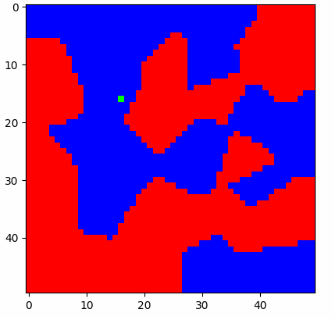
\includegraphics[scale=.75]{dopaje_50.png}
    \caption{Nanocristal dopado al 50\%.}
    \label{dopaje}
\end{figure}
El área obtenida de cada material tanto base como dopaje se interpreta como nanómetros cuadrados y la partícula verde que representa el flujo eléctrico atraviesa la muestra en diagonal a una velocidad constante siempre y cuando no detecte dopaje, si es así y encuentra dopaje entonces la velocidad de la partícula sera aumentada ya que un dopaje indica mejoramiento en velocidad pero a costa de menos pureza del material base.

\subsection{Resultados}
Los resultados del presente trabajo se graficaron en distintas representaciones debido a que los fenómenos estudiados fueron tanto la velocidad del flujo eléctrico así como el tamaño del cristal de cada muestra respecto a cada porcentaje del semiconductor.
El gráfico \ref{im1} muestra como varió el tamaño del cristal del material base respecto se iba variando la probabilidad del dopaje del semiconductor.
\begin{figure}[h!]
    \centering
    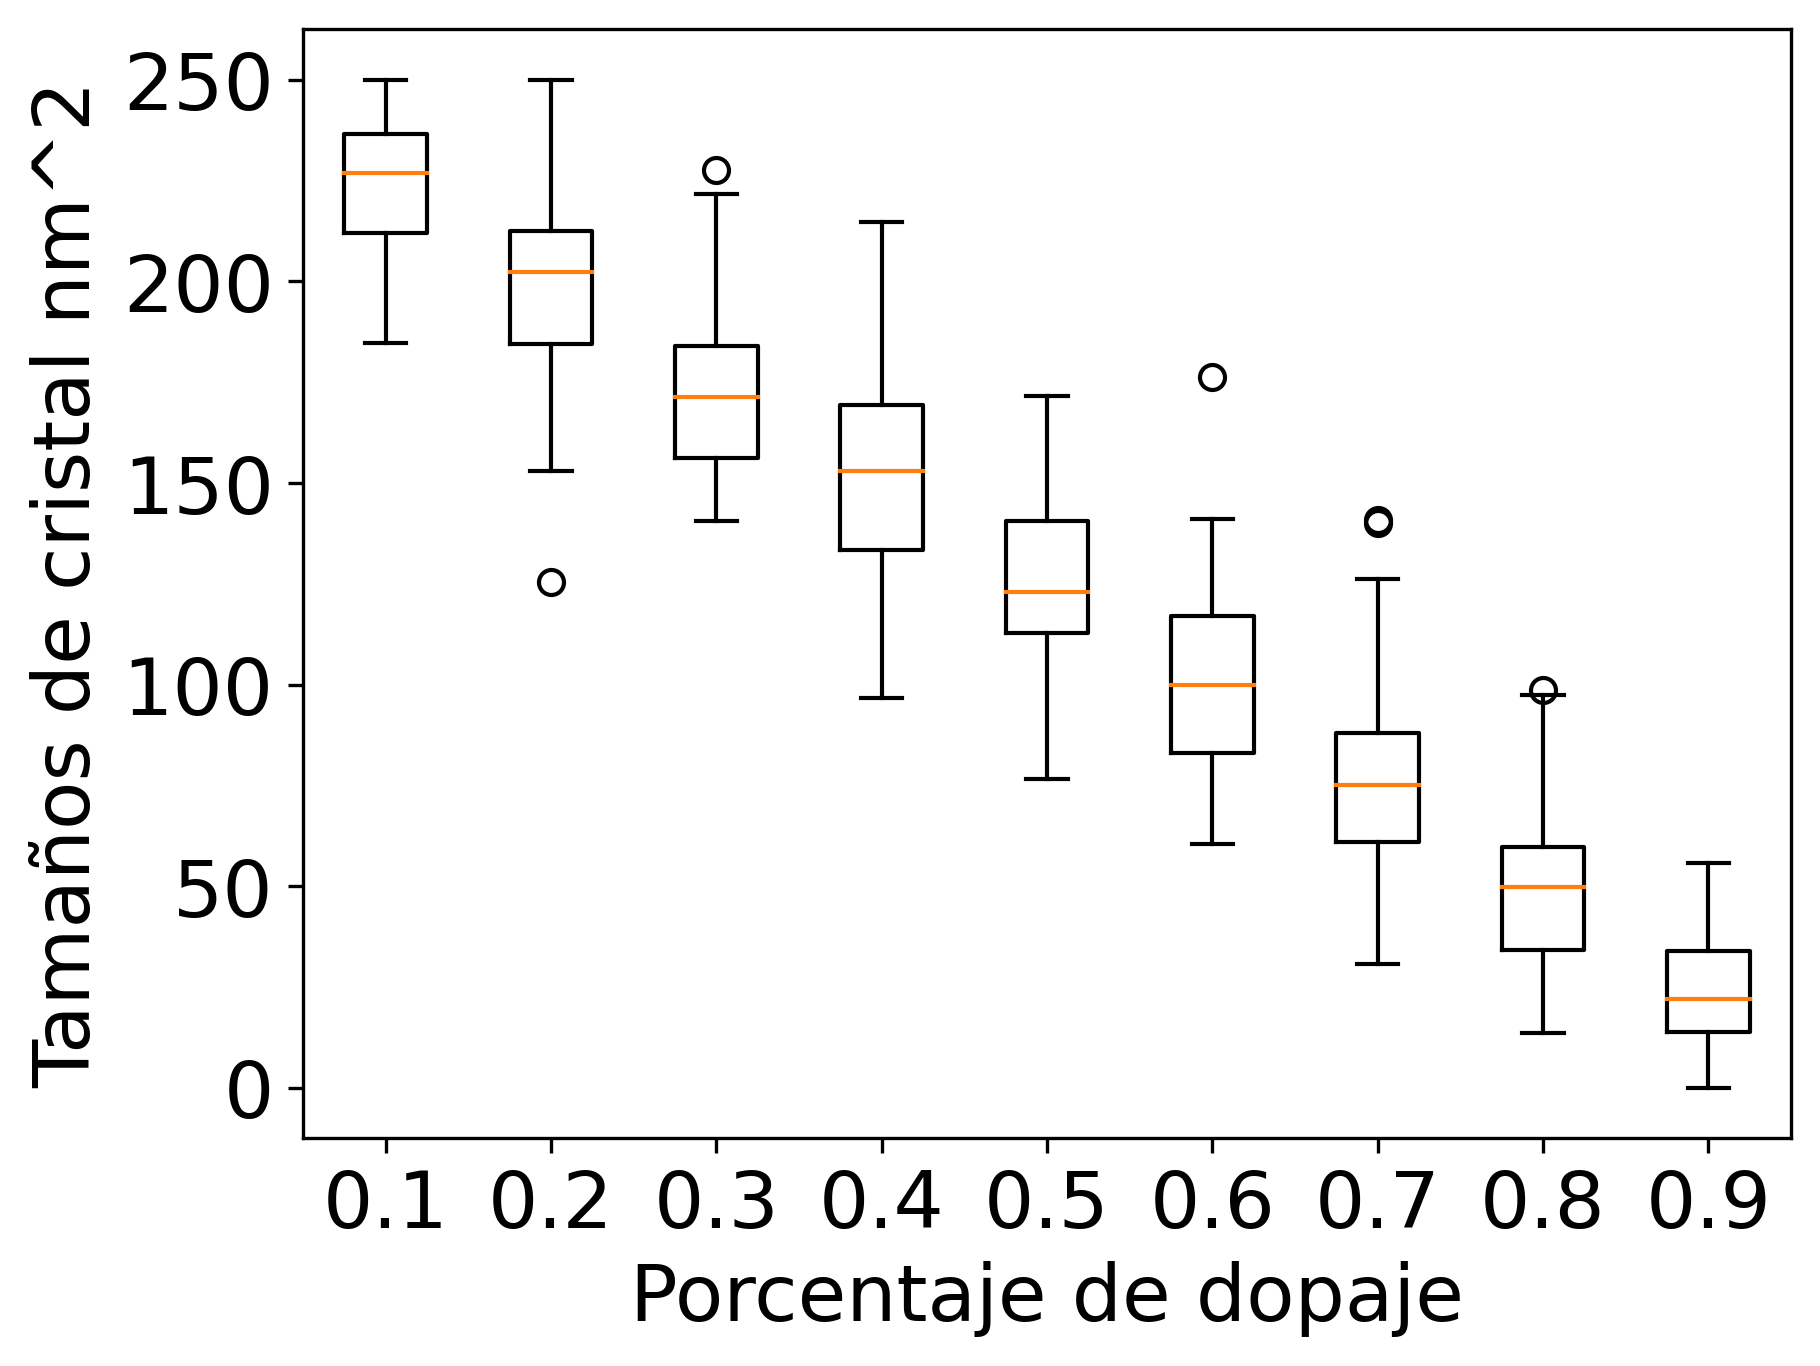
\includegraphics[scale=.5]{cris_porc.png}
    \caption{Gráfico caja bigote del tamaño del cristal base respecto al porcentaje de dopante.}
    \label{im1}
\end{figure}

La siguiente figura \ref{im2} al igual que la anterior analiza el tamaño del cristal solo que ahora se promediaron los valores recaudados y se realiza una comparativa entre el tamaño de cristal de base (linea roja) y el dopaje (linea azul).
\begin{figure}[h!]
    \centering
    \includegraphics[scale=.5]{tamaño_porc_tiem.png}
    \caption{Comparación tamaños de cristal base y dopante.}
    \label{im2}
\end{figure}

Por último la figura \ref{im3} muestra diagramas de violín y caja bigote combinados de como se vio afectado el tiempo o pasos en que terminó el flujo eléctrico de atravesar la muestra teniendo un tiempo máximo de 50 pasos. 
\begin{figure}[h!]
    \centering
    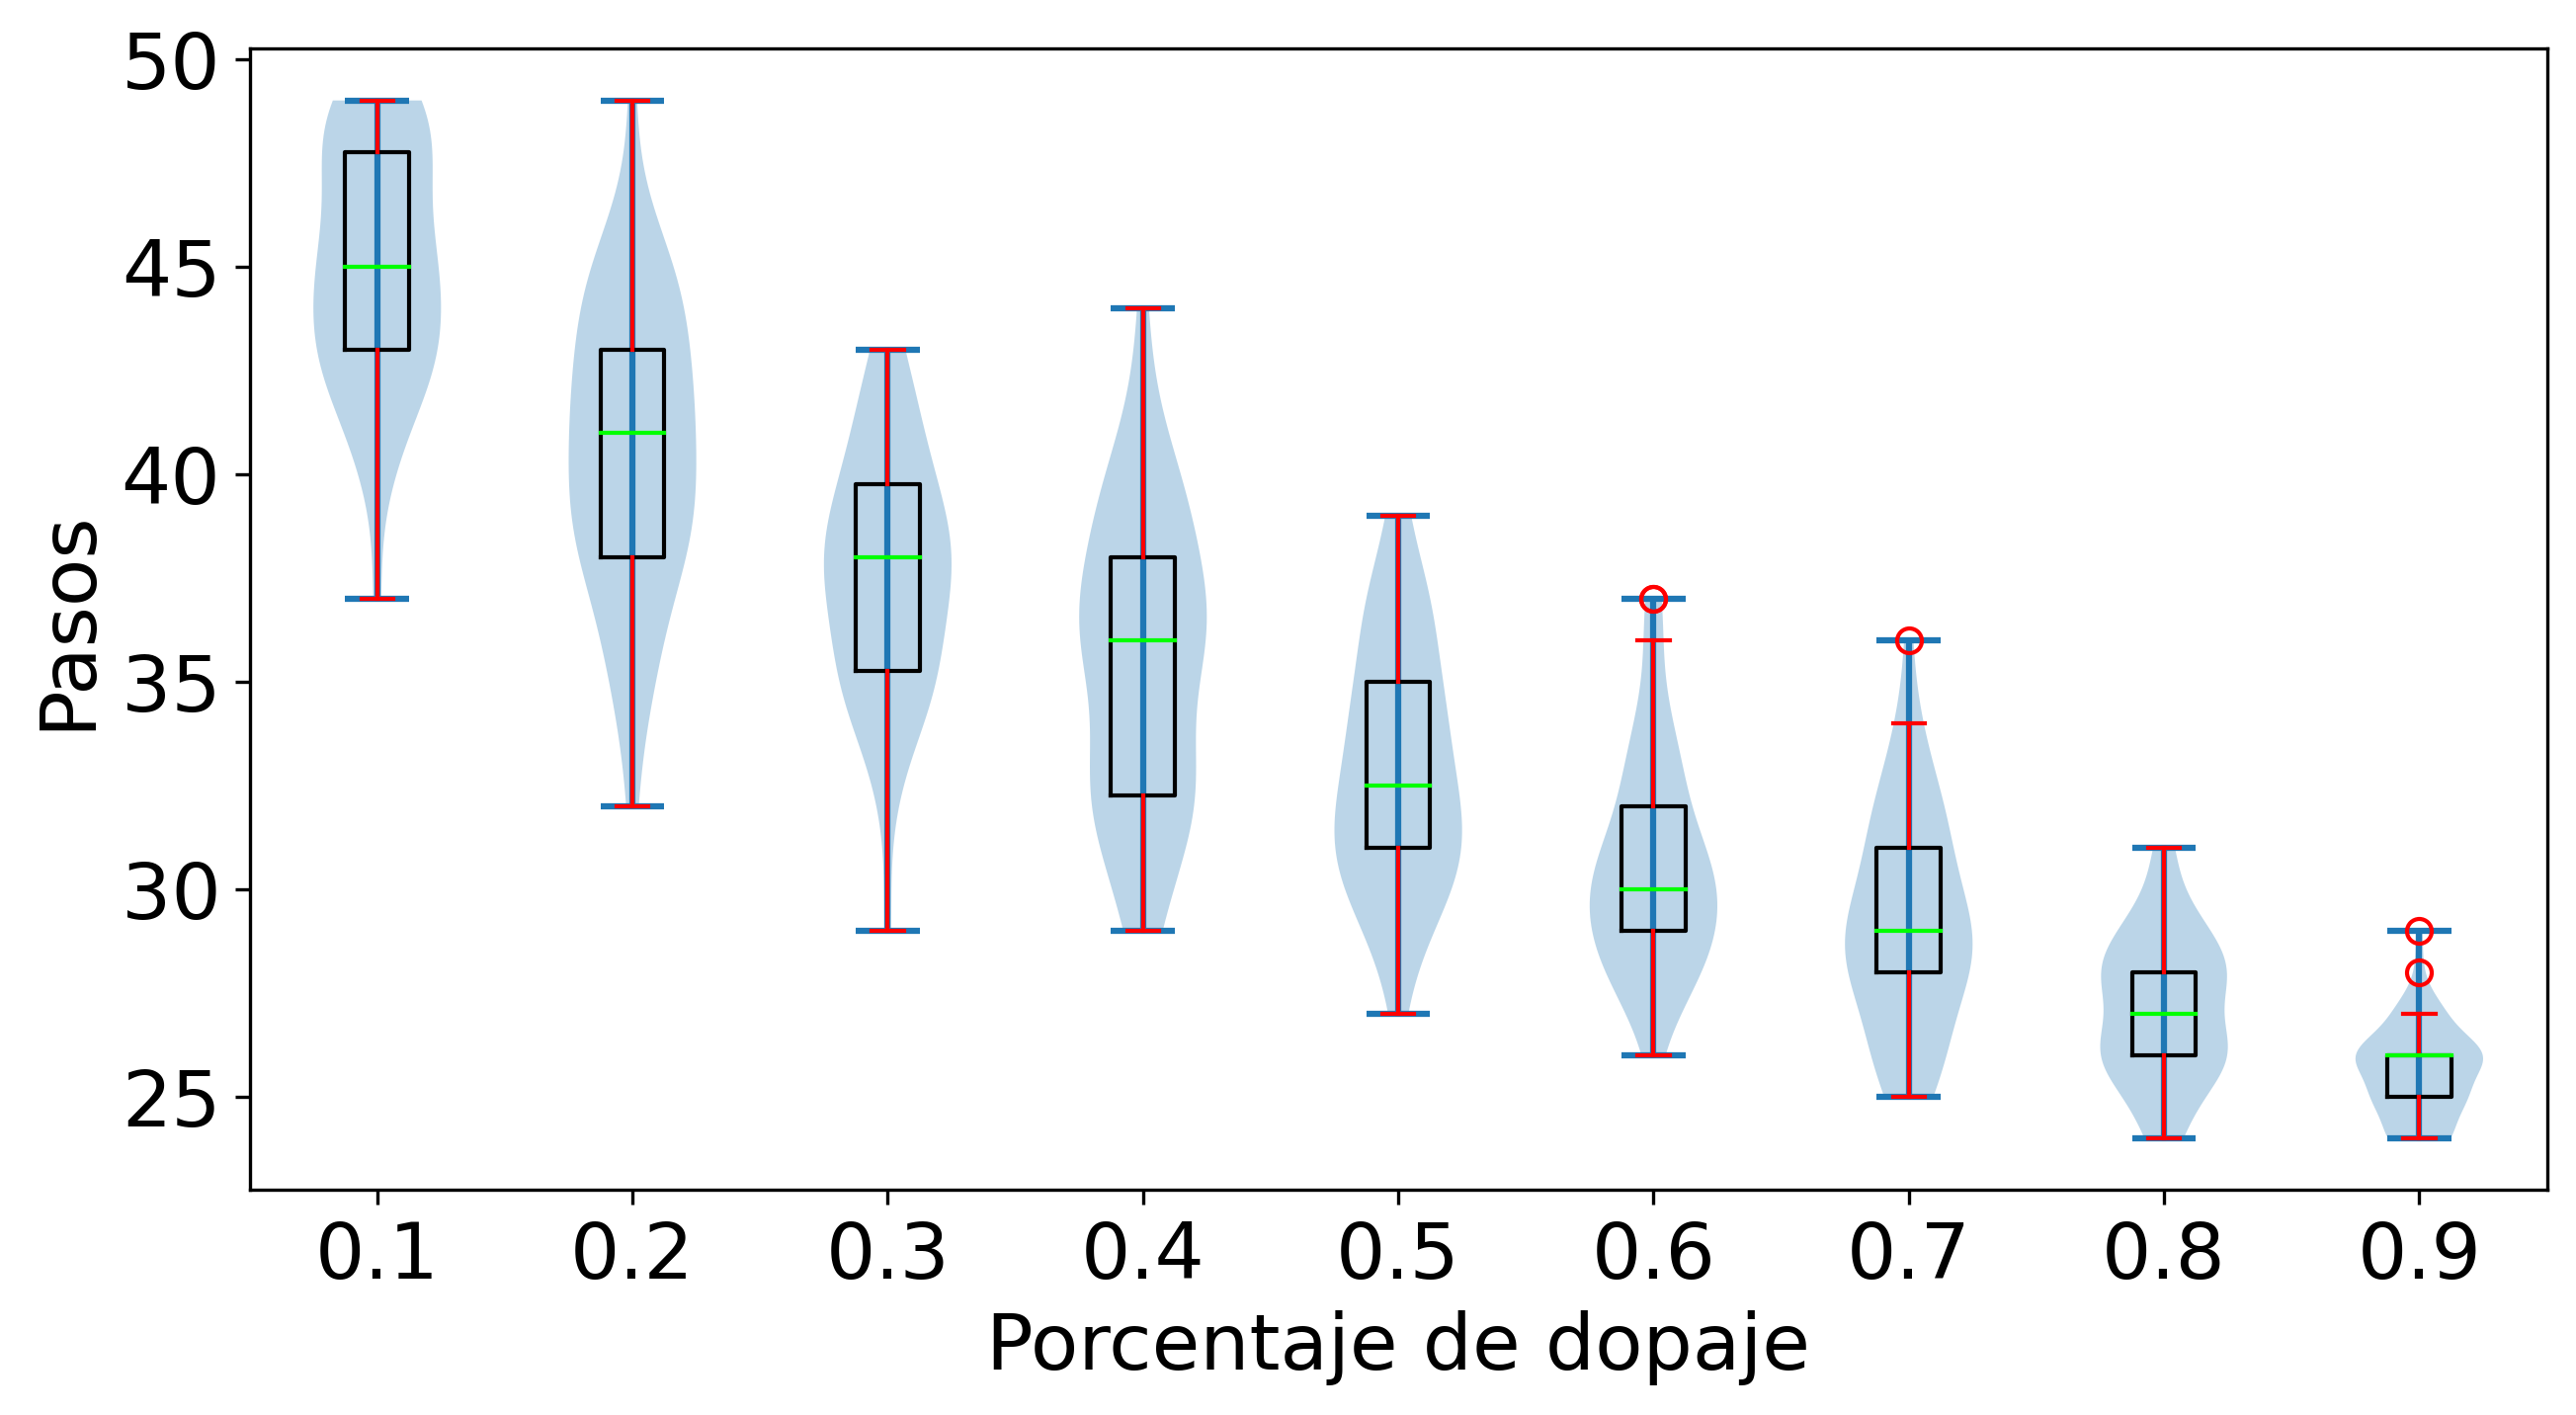
\includegraphics[scale=.38]{tiempo_porc.png}
    \caption{Velocidad del flujo eléctrico por porcentaje.}
    \label{im3}
\end{figure}


Los datos de los gráficos anteriores son mostrados en la tabla \ref{tab1} que muestra las probabilidades que se variaron en el experimento, los tamaños de cristal entre el material base y dopante y por ultimo el tiempo en pasos que tardo en recorrer la muestra teniendo un máximo de 50.
\begin{table}[H]
    \centering
    \caption{Tabla de tamaños de cristal y velocidad por probabilidad de dopaje.}
    \input{Datos}
    \label{tab1}
\end{table}

La última tabla \ref{statisc} obtenida, recauda los datos e información estadística de la gráfica \ref{im3}, en esta se puede encontrar los promedios por porcentajes, así como la varianza, asimetría y curtosis. 
\begin{table}[H]
    \centering
    \caption{Tabla estadística.}
    \scalebox{1}{
    \begin{tabular}{|c|c|c|c|c|}
       \hline
       Dopaje & Promedio & Varianza & Asimetría &Curtosis\\
       \hline\hline
       0.1& 44.3&8.948& -0.561 &-0.497\\
       \hline
       0.2&40.9&12.295& -0.111& -0.746\\
       \hline
       0.3&37.5&13.642& 0.456& 0.048\\
       \hline
       0.4&35.2&9.533& 0.327& 0.245\\
       \hline
       0.5&32.4&9.231& 0.981& 1.269\\
       \hline
       0.6&31.1&8.354 & 0.197&-0.158\\
       \hline
       0.7&28.8&5.171& 0.413& -0.277\\
       \hline
       0.8&27.1&2.173& 0.598& 1.299\\
       \hline
       0.9&25.3&1.724& 1.398& 2.396\\
       \hline
    \end{tabular}}
    \label{statisc}
\end{table} 

\section{Conclusiones}
En base a los resultados se puede concluir que la velocidad dependerá siempre del porcentaje que sea agregado de dopante ya que el flujo o conductividad será mas rápido aunque la pureza del material tiende a disminuir drásticamente, pero tal como se muestra en la figura \ref{im2} ocurre un cruzamiento de las lineas de los tamaños promedios del cristal, así que para mantener una buena proporción de pureza y dopante lo ideal es el 50\% de impurezas en la muestra para tener una buena conducción eléctrica que se observa en la tabla \ref{tab1} en la probabilidad de $0.5$. 

\subsection{Trabajo a futuro}
Como trabajo a futuro, la simulación puede ser ampliada para que la muestra admita 2 o 3 impurezas más, y aunado a esto realizar una variante de la dimensión de la muestra ya que en este estudio fue fija esa condición, de igual manera se podrían estudiar efectos de como se vería afectada la conducción térmica.

\bibliographystyle{plainnat}
\bibliography{sample}

\end{document}
